
     Relembrando, deseja-se uma turbina hidráulica que possui as seguintes características: operando em água, de massa específica ($\rho$) de $1000\;kg/m^3$, altura de queda ($H$) de 342 m, vazão ($Q$) de $2,23\;m^3/s$ e velocidade de rotação ($n$) de $300\;rpm$.

    \noindent
    \textbf{Dados adicionais}: \\
    Diâmetro do injetor ($D_i$): 0,20 $m$. \\
    Diâmetro da tubulação ($D_t$): 0,750 $m$. \\
    Viscosidade cinemática da água ($\mu$): $1,00 \times 10^{-3}\; Pa\:.\:s$. \\
    Comprimento da tubulação ($L$): 1000 $m$ \\
    Rugosidade da tubulação ($e$): 0,00026 $m$


\section{Seleção do tipo de Turbina}

    Para a turbina com dimensões reais serão identificadas pelo subscrito ``p'', enquanto para a turbina modelo serão pelo subscrito ``m''. Para selecionar o tipo de turbina que operará com essas condições, deve-se calcular o coeficiente de forma do rotor $n_{qA}$ e verificar na \autoref{tab-na} a máquina que possui o melhor rendimento.


    Primeiro, transforma a velocidade de rotação ($n_p$) que está rotações por minuto para rotações por segundo, dividindo por 60, tem-se $n_p = 5\;rps$, para a unidade da equação \eqref{eq-na} ser coerente e ter o coeficiente na forma adimensional.
    A energia por unidade de massa que o fluido entrega para a máquina será $ Y_p = g \; H_p = 9,81 \; . \; 342 = 3\;335,02\;J/kg $. Aplicando a equação \eqref{eq-na}, resulta em:
    \begin{equation*}
        n_{qA} = 10^3 \; . \; 5 \; . \; \frac{2,23^{0,5}}{3\;355,02^{0,75}} = 16,94
    \end{equation*}

    Que se enquadra na máquina de melhor rendimento a turbina Pelton visto na \autoref{tab-na}, e reforçado pela \autoref{fig-camp}.


\section{Velocidade do jato d'água  na saída do injetor}

    \begin{figure}[htb]
        \centering
        \caption{ \label{fig-pelton} Representação esquemática da turbina Pelton.}
        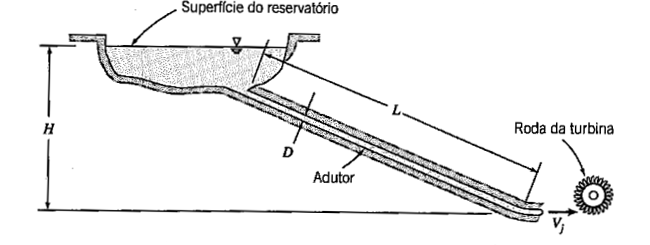
\includegraphics[scale=0.6]{images/turbina_pelton_fox.png}
        \legend{Fonte: Introdução a Mecânica dos Fluidos \cite{fox}}
    \end{figure}

    A \autoref{fig-pelton} representa um esquema da turbina pelton. Aplicando a equação \eqref{eq-perda_de_carga} de perda de carga total que será igual a equação de perda maior \eqref{eq-darcy},e considerando para um escoamento permanente, incompressível, completamente desenvolvido, no nível montante (1) e na saída do injetor (j), resulta em:
    \begin{equation*}
        \bigg( \cancel{\frac{p_1}{\rho}} + \cancelto{0}{\frac{V^2_1}{2}} + gz_1 \bigg) - \left( \cancel{\frac{p_j}{\rho}} + \frac{V^2_j}{2} + \cancelto{0}{gz_j} \;\;\: \right) = h_t = f \frac{L}{D}\: \frac{V_t^2}{2}
    \end{equation*}

    Como $p_1$ = $p_j$ = pressão atmosférica, e considerando o nível constante em 1 ($V_1 = 0$), e o nível de referência adotado na saída do injetor ($z_j$ = 0). Substituindo $z_1$ por $H$, é possível reorganizar a equação de cima para $V_j$:

    \begin{equation*}
        V_j^2 = 2gH - f \frac{L}{D} V_t^2
    \end{equation*}

    Em que $V_t$ é a velocidade do fluido dentro da tubulação e $V_j$ a velocidade do jato na saída do injetor. A velocidade do jato e a velocidade do tubo estão relacionados pela equação da continuidade: $A_t\: V_t = A_i \: V_j$. Assim, $V_t =  \frac{A_i}{A_t} \: V_j$ = $\left(\frac{D_i}{D_t} \right)^2 \: V_j$. Substituindo na equação de cima e reorganizando novamente para $V_j$, resulta em:

    \begin{equation} \label{eq-jato}
        V_j = \left[ \cfrac{2gH}{\left\{1 + f\cfrac{L}{D_t} \left(\cfrac{D_i}{D_t} \right)^4 \right\}} \right]^{\frac{1}{2}}
    \end{equation}

    A equação \eqref{eq-jato} fornece a velocidade do jato na saída do injetor já com a correção das perdas de carga na tubulação de adução, pois a perda de carga depende do comprimento da tubulação ($L$), o diâmetro da tubulação ($D_t$), o diâmetro interno do injetor ($D_i$) e altura de queda ($H$) e o fator de atrito $f$.

    Para calcular o fator de atrito $f$ foi utilizado a equação \eqref{eq-colebrook} de Colebrook, no entanto esta equação depende da rugosidade relativa e do número de Reynolds, e o número de Reynolds depende da velocidade da tubulação ($V_t$), mas não temos essa velocidade.

    Para resolver esse problema, foi proposto uma resolução através iteração, primeiro atribuiu-se um valor para a velocidade do jato sem a perda de carga, que é igual à $V_{j,i} = \sqrt{(2gH)} = 81,91 m/s$. Com esta velocidade inicial, podemos determinar a velocidade da tubulação $V_t$ através da equação da continuidade, logo em seguida calcula-se o número de Reynolds com a equação \eqref{eq-reynolds} para determinar o fator de atrito com a equação \eqref{eq-darcy} e logo em seguida aplica a equação \eqref{eq-jato} para determinar a nova velocidade do jato e repetir todo o processo, conforme está ilustrado no fluxograma à seguir:

    \begin{figure}[htb]
        \centering
        \caption{\label{fig-fluxo} Fluxograma representando o processo iterativo}
        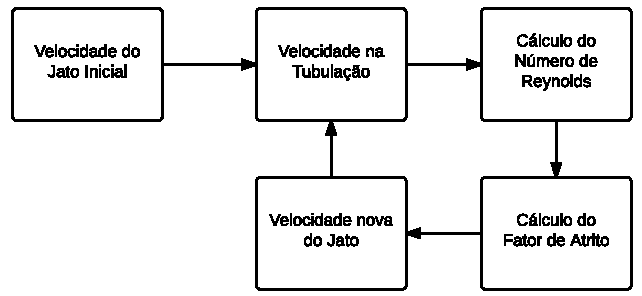
\includegraphics[scale=1]{images/fluxograma.pdf}
        \legend{Fonte: Figura elaborada pelos autores.}
    \end{figure}

    % \lstinputlisting[language=Python]{iteracao.py}

    % \begin{equation*}
    %
    % \end{equation*}

    Para executar o fluxograma da \autoref{fig-fluxo}, foi realizado pelos autores um programa computacional na linguagem de programação Python que se encontra no \autoref{ap-python}. O resultado da velocidade de saída do jato d'água $(V_j$) para uma tubulação feita de ferro fundido, e portanto, rugosidade ($e$) de 0,00026 $m$, convergiu para: $\mathbf{78,31\:} m/s$.

    \section{A velocidade absoluta do fluido na entrada do rotor}

    \begin{figure}[htb]
        \centering
        \caption{\label{fig-pelton_white} Velocidade do fluido na entrada do rotor}
        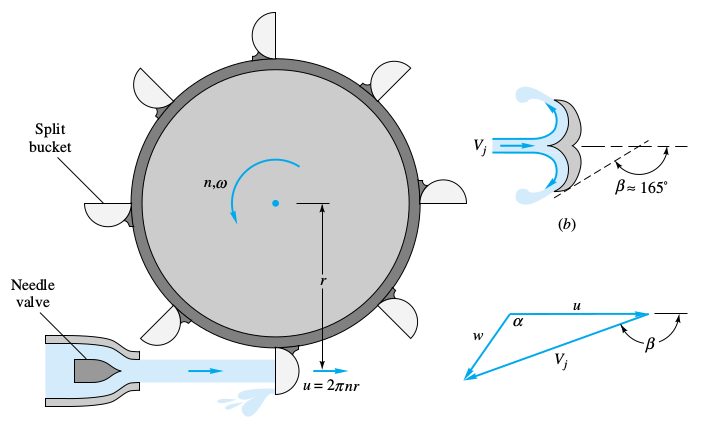
\includegraphics[scale=0.5]{images/pelton_turbine.png}
        \legend{Fonte: Fluid Mechanics \cite{white}.}
    \end{figure}
    A \autoref{fig-pelton_white} representa o funcionamento da turbina Pelton proveniente do jato d'água e demostra o triângulo de velocidades fornecido para um ângulo arbitrário $\beta$.

    Para um bocal perfeito, a velocidade do jato sem a perda de atrito seria a velocidade $V_j = 78,31 \: m/s$, no entanto considerando o bocal com superfícies irregulares, então a velocidade do jato corrigida será $V_{j,c} =  C_v \: V_{j}$, onde o coeficiente de velocidade ($C_v$) é usado e varia entre $0,92 \leq C_v \leq 0,98$. Considerando uma condição típica de trabalho, que é de um ângulo ($\beta$) de $160^{\circ}$, e $C_v$ igual à 0,94, ou seja, uma perda de 6\% segundo Frank White \cite{white}. Portanto a velocidade do jato d'água corrigida ($V_{j,c}$) é de  $73,61\: m/s$.

\section{Diâmetro do rotor da turbina modelo}

    \begin{figure}[htb]
        \centering
        \caption{\label{fig-rendimento} Eficiência de uma turbina de ação}
        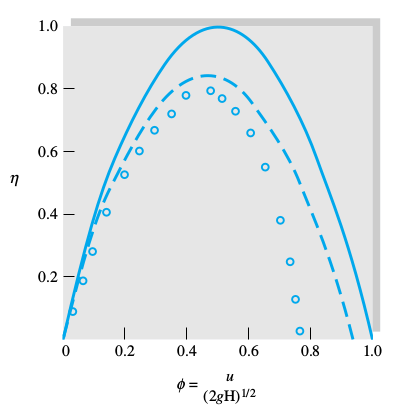
\includegraphics[scale=0.5]{images/eficiencia_pelton.png}
        \legend{Fonte: Fluids Mechanics \cite{white}.}
    \end{figure}

    A \autoref{fig-rendimento} representa a eficiência ($\eta$) de uma turbina de ação, como é a turbina Pelton para diferentes valores da relação da velocidade absoluta do rotor ($u$), com a velocidade absoluta do jato d'água sem a correção $V_j$, para essas condições de trabalho o máximo rendimento é ($\eta_{max}$) = 85\%, e $\phi$ é igual à 0,47 \cite{white}.

    Sendo assim, a velocidade absoluta do rotor será:
    \begin{equation*}
        u = 0,47 \; . \; V_{j,c} = 0,47 \; . \; 73,61 = 34,60 \: m/s
    \end{equation*}

    O diâmetro do rotor do protótipo pode então ser calculado através da equação básica da velocidade angular $u = 2 \pi r n = \pi D n$ e rearranjando para o diâmetro, tem-se:

    \begin{equation*}
        D_p = \frac{u}{\pi \; . \; 5} = 2,20\: m
    \end{equation*}

    Como o fator de escala é $k_G = \frac{D_p}{D_m} = 10$, o diâmetro do rotor no modelo é, utilizando a equação \eqref{eq-geometrica}:

    \begin{equation*}
        D_m = \frac{D_p}{k_G} = \frac{2,20}{10} = 0,220\:m \mbox{ ou } 220\: mm
    \end{equation*}

\section{A velocidade de rotação da turbina modelo}

    A altura de queda também será de 10 (dez) vezes menor, desse modo:
    \begin{equation*}
        H_m = \frac{H_p}{10} = \frac{342}{10} = 34,2\:m \implies Y_m = g \: . \: H_m = 9,81 \: . \: 34,2 = 335,5\: J/kg
    \end{equation*}

    Como as grandezas biunitárias são iguais para máquinas de fluxo semelhantes, com base na equação \eqref{eq-vel-bi} pode-se escrever:
    \begin{equation*}
        \begin{split}
            n_{11} &= \frac{n_m \: D_m}{Y_m^{\rfrac{1}{2}}} = \frac{n_p \: D_p}{Y_p^{\rfrac{1}{2}}} \; \therefore \\
            n_m &= n_p \: \frac{D_p}{D_m}\: \left(\frac{Y_m}{Y_p} \right)^{\rfrac{1}{2}} = 5\; \frac{2,20}{0,220} \left( \frac{335,5}{3355,02} \right)^{\rfrac{1}{2}} \; \therefore \\
            n_m &= 15,81 \: rps \mbox{ ou } 948,68\: rpm
        \end{split}
    \end{equation*}

\section{A potência no eixo da turbina modelo}

    Considerando as perdas na instalações ignoradas e um rendimento de, $\eta_p = 0,85$, a potência do protótipo pode ser calculada pela equação abaixo:
    \begin{equation*}
        P_{ep} = \rho \, . \, Q_p \, . \, Y_p \, . \, \eta_p = 1000 \, . \, 2,23 \, . \, 3355,02 \, . \, 0,85 = 6359,4 \: \mbox{kW}
    \end{equation*}

    E considerando um rendimento invariável entre modelo e protótipo, o modelo também operando com água, a equação \eqref{eq-pot-bi} permite estabelecer:
    \begin{equation*}
        \begin{split}
            P_{e11} &= \frac{P_{em}}{D_m^2 \: . \: Y_m^{\rfrac{3}{2}}} = \frac{P_{ep}}{D_p^2 \: . \: Y_p^{\rfrac{3}{2}}} \; \therefore \; P_{em} = P_{ep} \; \left( \frac{D_m}{D_p} \right)^2 \left( \frac{Y_m}{Y_p} \right)^{ \! \rfrac{3}{2}} \; \therefore  \\
            P_{em} &= 6359,4 \left( \frac{0,220}{2,20} \right)^2 \left( \frac{335,5}{3355,02} \right)^{\rfrac{3}{2}} = 2,01 \; \mbox{kW} 
        \end{split}
    \end{equation*}
